The selected regional spectra are summarized in Table~\ref{tab:random-spectra}. Here $\Delta=T^2-4D$. The lower regions are stable nodes, the middle regions unstable foci and the upper regions stable foci. In AFM and FM, the middle-zone discriminant is close to zero, making its classification sensitive to coefficient changes. These regional checks do not establish the applicability of a theorem without checking its remaining hypotheses.
\begin{table*}[t]
\centering
\caption{Regional trace $T$, determinant $D$ and discriminant $\Delta$ for the selected PWA candidates. Values are rounded; full-precision coefficients and numerical checks are archived with the models.}
\label{tab:random-spectra}
\begin{tabular}{llrrr}\toprule
Regime & Region & $T$ & $D$ & $\Delta$ \\\midrule
AM & lower & $-2.170831$ & $0.784727$ & $1.573600$ \\
AM & middle & $0.513096$ & $0.373041$ & $-1.228897$ \\
AM & upper & $-0.374896$ & $0.206460$ & $-0.685295$ \\
AFM & lower & $-15.298470$ & $1.841114$ & $226.678720$ \\
AFM & middle & $1.299833$ & $0.422429$ & $-0.000151$ \\
AFM & upper & $-0.635047$ & $0.516281$ & $-1.661837$ \\
FM & lower & $-33.605867$ & $3.996778$ & $1113.367175$ \\
FM & middle & $0.838872$ & $0.176338$ & $-0.001647$ \\
FM & upper & $-0.128202$ & $0.100218$ & $-0.384438$ \\\bottomrule
\end{tabular}
\end{table*}

At the prescribed folds, matching residuals and $|\log M|$ are below $10^{-13}$. Numerical finite differences support nonzero $G_{ss}$ and $G_I$ for the chosen four-segment return map: approximately $(-260,-200)$ for AM, $(-2814,-16.0)$ for AFM, and $(-6591,-27.2)$ for FM. These are step-dependent numerical estimates, not a proof; AM has a small minimum crossing speed ($3.66\times10^{-4}$ in the model units), and several larger finite-difference steps fail to resolve the map. For AM, AFM and FM, respectively, the minimum absolute normal speeds at the four fold crossings are $3.6640\times10^{-4}$, $8.7669\times10^{-3}$ and $2.8399\times10^{-3}\,\mu\mathrm M\,\mathrm{s}^{-1}$. At section-coordinate steps $10^{-6}$ and $3\times10^{-7}$, the estimated $G_{ss}$ values are $(-260.20,-261.64)$, $(-2814.39,-2814.19)$ and $(-6590.73,-6590.58)$; at input steps $10^{-8}$ and $10^{-9}\,\mu\mathrm M$, $G_I$ is $(-200.15,-200.12)$, $(-16.01663,-16.01661)$ and $(-27.16601,-27.16599)$. Each perturbed route passed sampled residence and crossing-direction checks; these checks do not prove first crossing throughout each segment. Full-precision coefficients, input lists, failed steps and scripts are recorded in the accompanying reproducibility files. We do not claim global cycle uniqueness or completeness.

Figure~\ref{fig:random-cycles} compares sampled cycle extrema and periods. The selected FM model underestimates $C_{\max}$ at lower inputs and overestimates it at higher inputs, so period agreement alone does not establish faithful FM amplitude modulation. At one AM holdout input the original matching search failed; a separate IVP-seeded matching solve found a stable physical cycle. This confirms a numerical search failure for that point, not general completeness of the search.
The numerically continued equilibria and portions of stable and unstable
cycle branches are also compared with LR in Fig.~\ref{fig:random-bifurcation};
gaps in the PWA branches indicate the limits of the continuation, not proven
absence of cycles.
\begin{figure*}[t]
\centering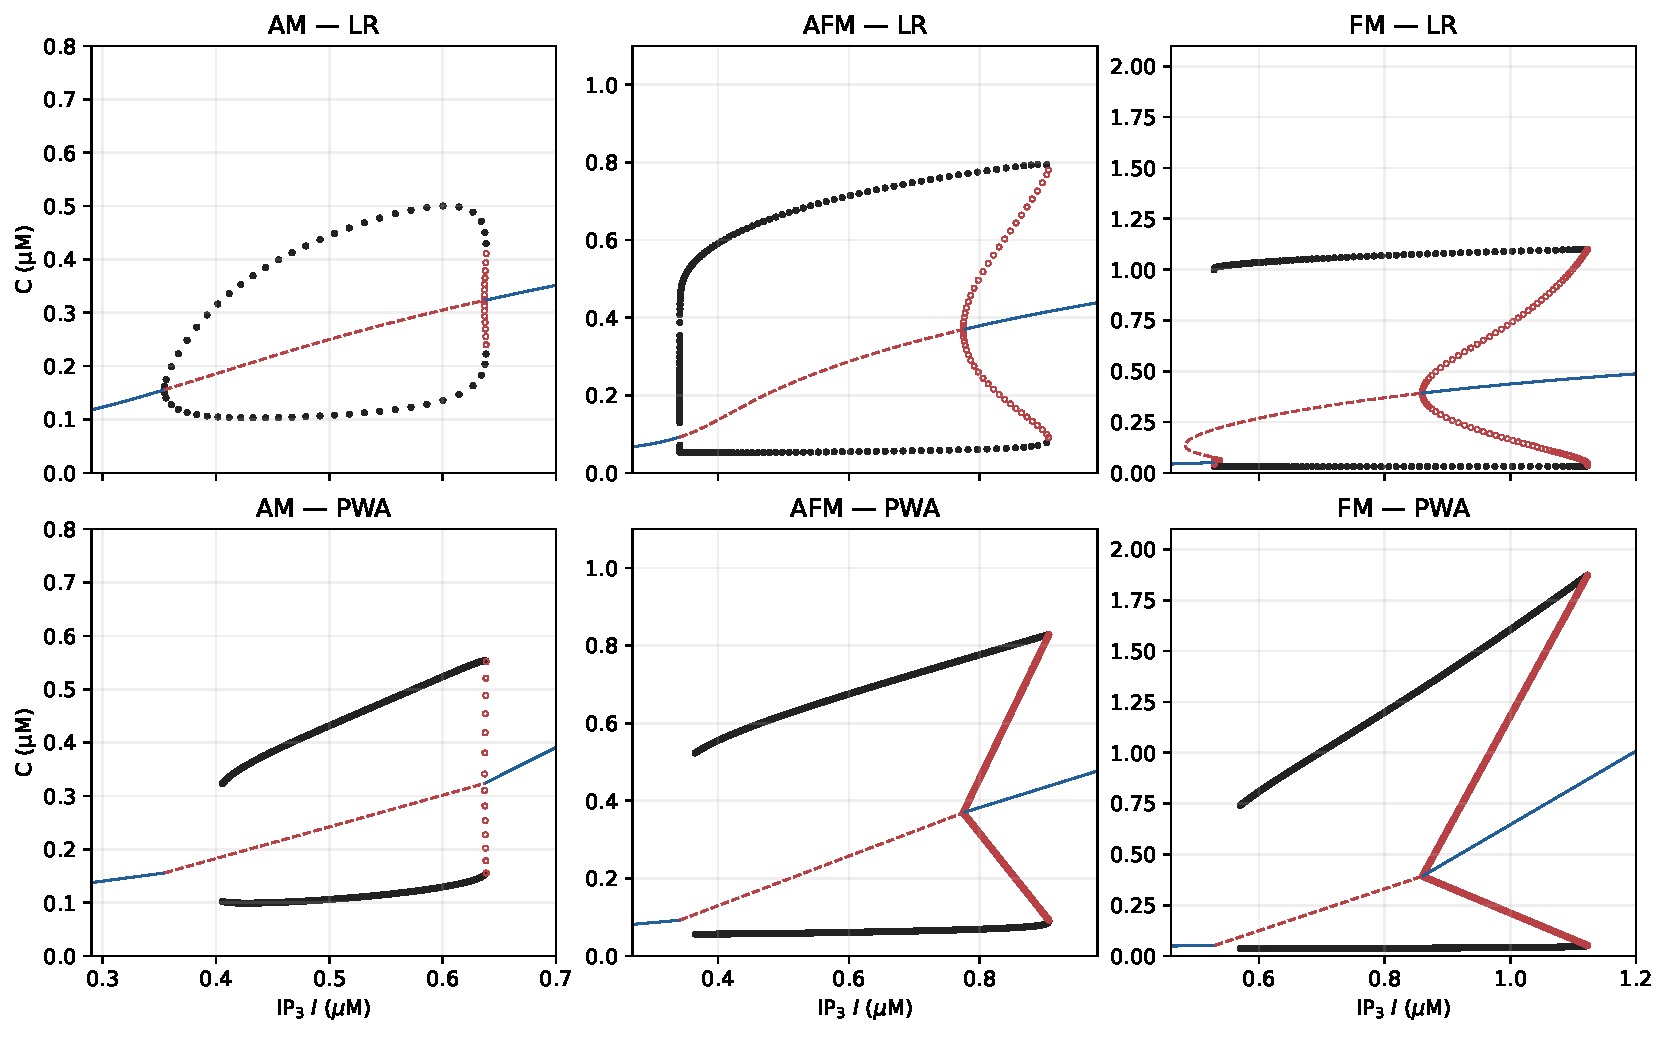
\includegraphics[width=\textwidth]{figures/random_selected_bifurcations.pdf}
\caption{Reference LR (top) and selected PWA fields (bottom). Blue solid and
red dashed lines denote stable and unstable equilibrium segments. Filled black
and open red markers show numerically obtained stable and unstable cycle
extrema, respectively. Each model is shown only over the computed portions;
missing PWA branches do not establish nonexistence.}
\label{fig:random-bifurcation}
\end{figure*}
\begin{figure*}[t]
\centering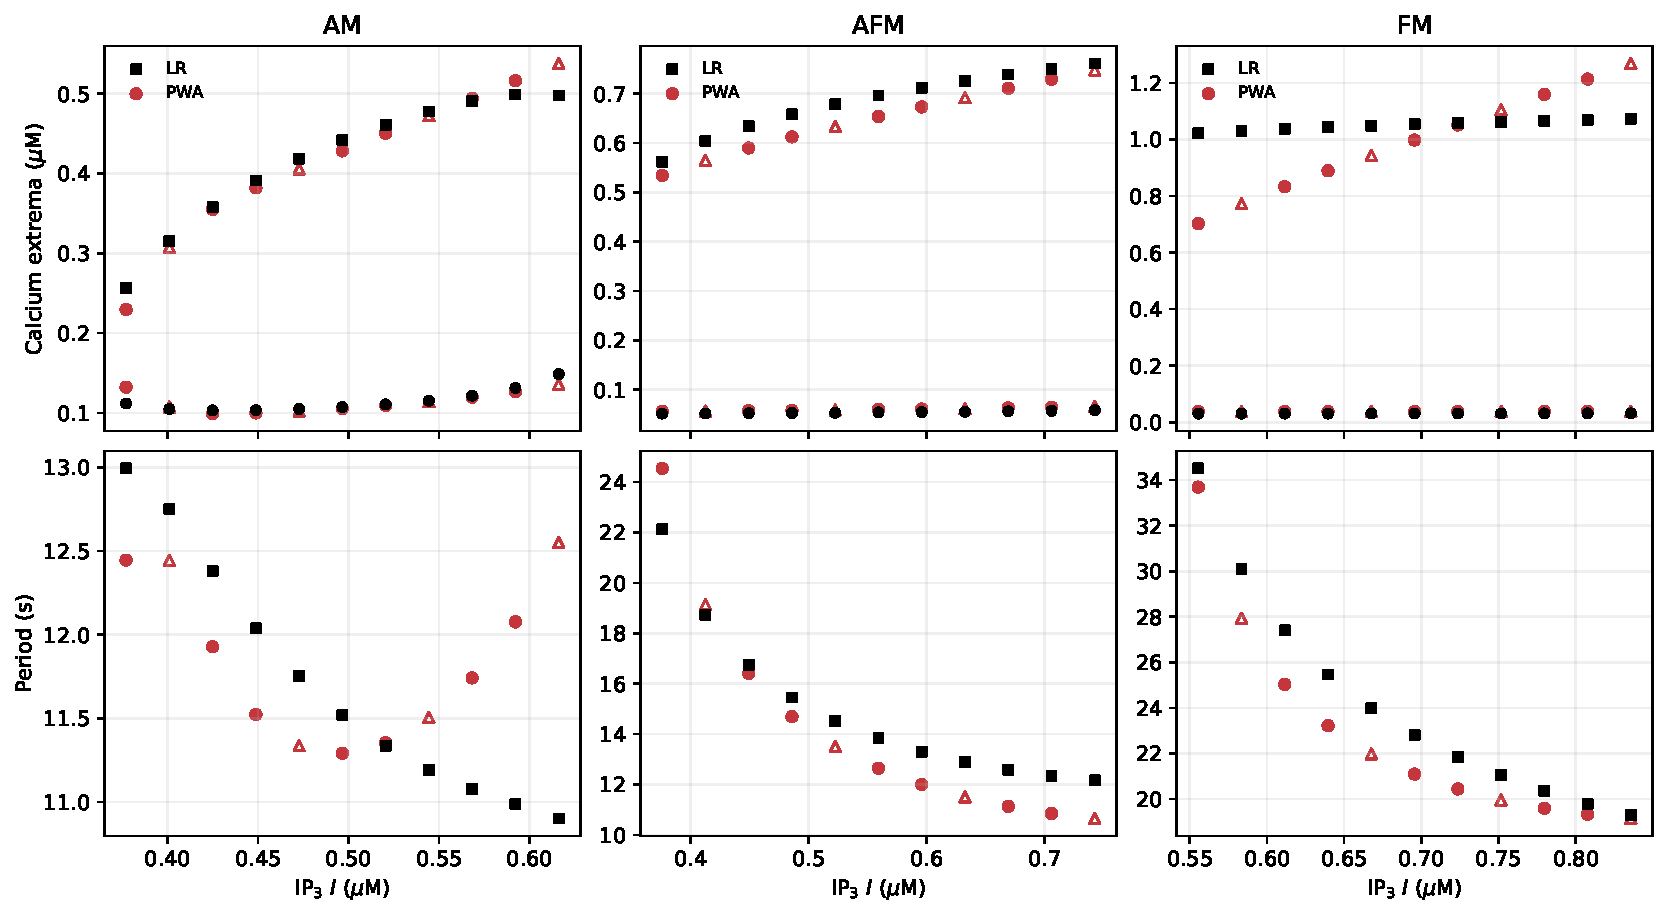
\includegraphics[width=\textwidth]{figures/random_selected_cycles.pdf}
\caption{Calcium extrema and period at seven fitting and four holdout inputs. Black circles and squares denote LR minima and maxima, respectively; red filled circles denote PWA fitting points and open triangles denote holdout points. The additional IVP-seeded AM holdout check is included. Points do not constitute a continuous bifurcation continuation.}
\label{fig:random-cycles}
\end{figure*}

Numerical continuation from each neutral orbit provides the partial four-segment branches in Fig.~\ref{fig:random-fold}. Continuation in one direction stopped after 2, 5 and 3 points for AM, AFM and FM, respectively, when independent integration could not be resolved; in the other direction AM stopped after 188 points on unresolved independent integration, whereas AFM and FM reached the 420-point budget. By solving for grazing of the lower switching line and switching itineraries, we additionally continued 6, 129 and 239 unstable upper-only cycles for AM, AFM and FM, respectively. The corresponding grazing inputs lie approximately $3.16\times10^{-9}$, $8.65\times10^{-5}$ and $2.17\times10^{-5}$ $\mu$M below the prescribed fold inputs. AM ordering is especially sensitive to numerical precision. These numerical endpoints do not imply that the branches terminate there.
\begin{figure*}[t]
\centering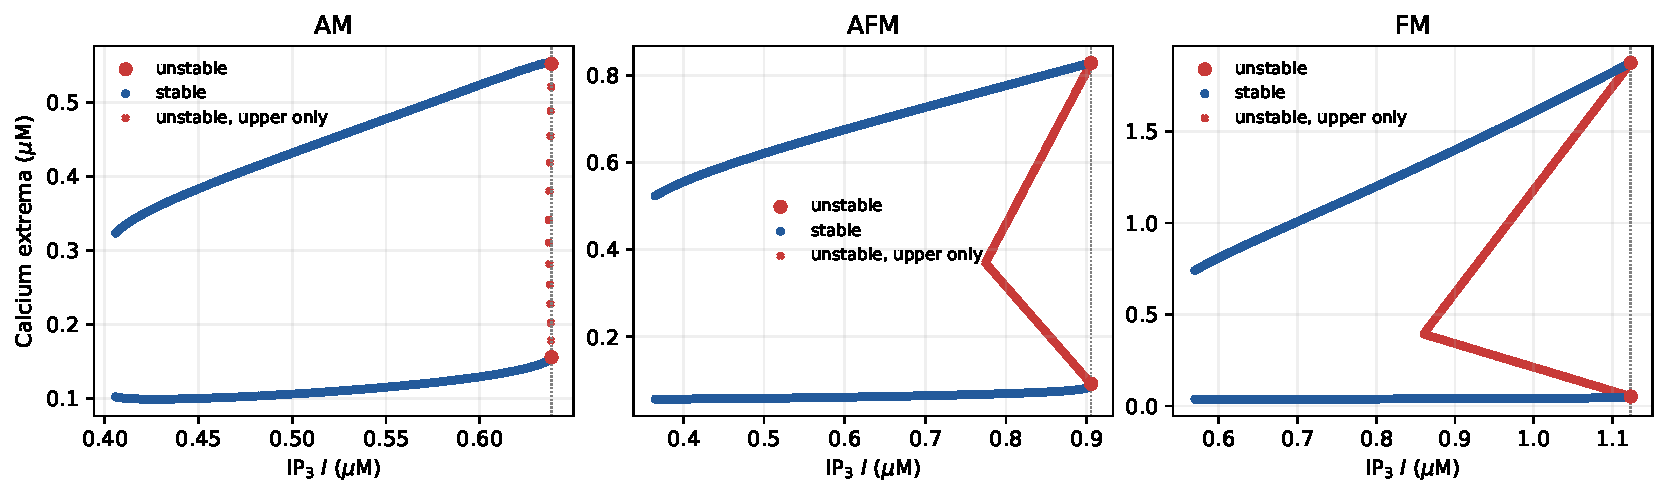
\includegraphics[width=\textwidth]{figures/random_selected_fold_continuation.pdf}
\caption{Computed portions of PWA cycles near the imposed fold input (dotted line). Blue and red circles denote stable and unstable cycles crossing both thresholds, respectively; red crosses denote unstable cycles crossing only the upper threshold. Only sampled positive-calcium orbits are shown. The continuation is finite and does not prove branch completeness.}
\label{fig:random-fold}
\end{figure*}
